\documentclass[12pt,fleqn]{article}\usepackage{../common}

\begin{document}
Ders 23 

Bu ders Laplace Transformlarinin son dersi, ayni zamanda, yeni bir girdi
fonksiyonunu gorecegiz -- birim d�rt� (unit impulse) fonksiyonlari. Bu
fonksiyonlar ne ise yarar? Mesela tum paranizi bankaya koydunuz, sonra
yarisini cektiniz, vs. Bu tur hesaplar d�rt� fonksiyonu ile yapilir. Peki
d�rt� nedir? D�rt�, mesela bir objeye bir zaman surecinde $f(t)$ kuvveti
uyguladigimizda,

\[ f(t) \textit{ durtu } = \int _{a}^{b}f(t)dt \]

Eger $f(t)$ sabit ise, ustteki su hale gelir

\[ Durtu = F \cdot (b-a) \]

Peki guc derken nasil bir sistemden bahsediyoruz? Mesela

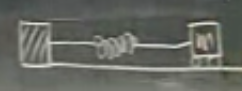
\includegraphics[height=2cm]{23_1.png}

Bu sisteme sagdan, belli bir sure bir guc uyguladigimizi dusunelim, $f(t)$
bu iste. 

Bu sistemin davranisini Laplace Transform ile cozmek icin kuvveti nasil
modellerim? Diyelim ki 

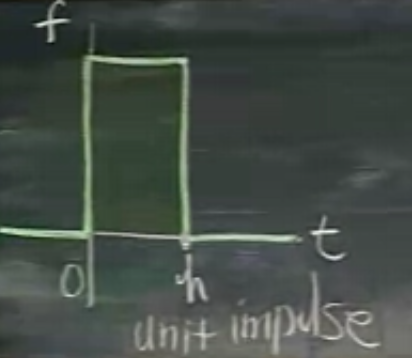
\includegraphics[height=3cm]{23_2.png}

0 aninda kuvvet uygulamasi basliyor, 0'dan yukari cikiyoruz, $h$ kadar
devam ediyor, sonra sifira iniyoruz. Eger bu d�rt�un, yani grafik altindaki
entegral alaninin 1 olmasini istiyorsak (ki d�rt� birim olabilsin), o zaman
kuvvet sifirdan $1/h$'ye yukselmeli. 

Yay sistemini modellersek (ve birim adim fonksiyonunu kullanirsak)

\[ y'' + y  = \frac{1}{h}u_{0h}(t) \]

Birim adim notasyonumuz, hatirlanacagi gibi, $a,b$ arasinda 1 olan bir
durum icin $u_{ab}$ idi, ama bu ornekte 1 degil, $1/h$'ye cikiyoruz, o
zaman her seyi $1/h$ ile carpariz.

Ustteki sistemi cozmek istiyorsak, sag tarafin Laplace Transformunu almamiz
lazim. Her seyi birim adim fonksiyonu ile yazalim, ve transformu yapalim

\[ \frac{1}{h} [ u(t) - u(t-h) ] 
\stackrel{\mathcal{L}}{\leadsto} \ \ ?
\]

Hatirlarsak

\[ u(t-a)g(t-a) \stackrel{\mathcal{L}}{\leadsto}  e^{-as}G(s) \]

O zaman iki ustteki

\[ = \frac{1}{h}[ \frac{1}{s} - \frac{e^{-hs}}{s} ]\]

Simdi su soruyu soralim: eger $h$ sifira giderse ne olur? Laplace Transform
ne olur? Elimizdeki birim d�rt� olduguna gore, $a,b$ araligi kuculdukce,
alan 1 kalmak zorunda oldugu icin kuvvet sonsuza gitmelidir. 

\[ \lim_{h \to 0} \frac{1-e^{-hs}}{hs} \]

$u=hs$ kullanalim, temiz olsun 

\[ \lim_{u \to 0} \frac{1-e^{-u}}{u} \]

Limite bakarsak bolum ve bolen ayni anda sifir oluyor, yani $0/0$
durumu. Bu istenen bir sey degil. Cozum nedir? Bazilari Taylor acilimi
yaparak serideki ilk birkac terimi usttekinin yerine gecirebilir. Ama
cogunuz bu noktada herhalde L'Hospital Kuralini kullanacaktir. Bolum ve
bolenin ayri ayri turevini aliriz,

\[ = \lim_{u \to 0} \frac{e^{-u}}{1} = 1\]

Basa donersek, 

\[ \frac{1}{h}u_{0h}(t) \leadsto \frac{1-e^{-hs}}{hs} \]

Ustteki $h \to 0$ iken 1' yaklasiyor.  










\end{document}
